% Version History
% 2020-10-27  	    Holger Graf
%                   Licence CC BY 4.0
%					Link: https://www.overleaf.com/latex/templates/thesis-template-microeconomics-at-fsu-jena/shqhkgcqtvsn
%					Accessed 18.01.2023
% 2023-02-01		Adapted by Ines Rieger
%					Licence CC BY 4.0
%					Lehrstuhl für Erklärbares Maschinelles Lernen
%					Universität Bamberg
% Please adapt this tex file for your thesis

\documentclass{xai-thesis}

\usepackage{graphicx}
\usepackage{setspace}
\usepackage{hyperref} % use \usepackage[hidelinks]{hyperref} to hide boxes
\usepackage[utf8]{inputenc} % depends on the font encoding that you are using
\usepackage[round]{natbib}

\usepackage{subcaption}

\input{math_commands.tex}

\begin{document}
% ----------------------------------------------------------------------------
% Details for the titlepage
% ----------------------------------------------------------------------------
\thesisTitle{AI-assisted estimation of wood knots in historic timber structures}
\thesisType{Master Thesis} % 'Master Thesis' or 'Bachelor Thesis'
\thesisAuthor{Pan, Junquan}
\thesisGrade{Master of Science in Digital Technologies in Heritage Conservation}
\thesisFirstSupervisor{Prof. Dr. Christian Ledig} % your supervising professor
\thesisSecondSupervisor{Dr.-Ing. Maria Chizhova} % if you are supervised by additional advisors, e.g phd students at the chair or a  supervisor in a company (write company after the name of the supervisor)
\thesisDate{\today}

% Print titlepage
\thesisMakeTitle

% ----------------------------------------------------------------------------
% Abstract
% ----------------------------------------------------------------------------
\clearpage
\pagenumbering{roman}
\pagestyle{plain}

\subsection*{Abstract}
Short summary of your thesis (max. 1 page) \ldots

\clearpage
\subsection*{Abstract}
Kurze Zusammenfassung Ihrer Abschlussarbeit (max. 1 Seite) \ldots

% ----------------------------------------------------------------------------
% Acknowledgements
% ----------------------------------------------------------------------------
\clearpage
\subsection*{Acknowledgements}
If you want to thank anyone (optional) \ldots

% ----------------------------------------------------------------------------
% Table of contents
% ----------------------------------------------------------------------------
\clearpage
%\thispagestyle{empty}
\tableofcontents

% ----------------------------------------------------------------------------
% List of figures/tables/acronyms
% ----------------------------------------------------------------------------
\clearpage
\phantomsection
\addcontentsline{toc}{section}{List of Figures}
\listoffigures
% --------------------------
\clearpage
\phantomsection
\addcontentsline{toc}{section}{List of Tables}
\listoftables
% --------------------------
\clearpage
\phantomsection
\addcontentsline{toc}{section}{List of Acronyms}
\section*{List of Acronyms}
\begin{tabular}{@{}ll}
AI & Artificial Intelligence\\
\end{tabular}

% ----------------------------------------------------------------------------
% Notation
% ----------------------------------------------------------------------------
\clearpage
\section*{Notation}
\input{math_notation.tex}

% --------------------------

% ----------------------------------------------------------------------------
% Contents
% ----------------------------------------------------------------------------
\cleardoublepage
\pagestyle{headings}
\pagenumbering{arabic}
\setcounter{page}{1}

% Hint: It is advisable to split the thesis into several tex files organized by sections. You can use thesis.tex as the main file and include any other tex file with \input(introduction.tex)

\section{Introduction}
\label{sec:intro}

\renewcommand\thesection{\arabic{section}}
\renewcommand\thesubsection{\thesection.\arabic{subsection}}





\newpage
\section{Theoretical foundation}
\label{sec:first}

\subsection{Analysis of the condition of historic wooden beams}
\label{subsec:first}

\subsection{Application of machine learning in related fields}
\label{subsec:second}



\newpage
\section{Methodology}
\label{sec_3}

\renewcommand\thesection{\arabic{section}}
\renewcommand\thesubsection{\thesection.\arabic{subsection}}

\textbf{General workflow}:
To accurately detect and estimate the wood knots on target wooden beam, the above roadmap(Figure~\ref{fig:process}) shows the general process of ideal workflow. The whole process is considered in terms of several frequently captured images, each image being processed through the segmentation and detection process, and all the images being composited as a final output when the capture is complete.

\begin{figure}[ht]
  \centering
   \includegraphics[width=1\textwidth]{Master Thesis/Images/Section_3/3-Process.jpg}
  \caption{Technology Roadmap}   
  \label{fig:process}
\end{figure}  




\subsection{Segmentation of wooden beams}
\label{sec_3:3.1}

\renewcommand\thesection{\arabic{section}}
\renewcommand\thesubsection{\thesection.\arabic{subsection}}


\textbf{Goal}:\\
To segment the detected surface of wooden beams, especially give the difference between the main surface and the others; (ideal output like Figure~\ref{fig:mock1})

\hspace*{\fill}


\begin{figure}[ht]
  \centering
    \begin{subfigure}[b]{0.4\textwidth}
      \centering
        \includegraphics[width=0.5\textwidth]{Master Thesis/Images/Section_3/Mock/3-Mock1.png}
    \end{subfigure}
    \begin{subfigure}[b]{0.4\textwidth}
      \centering
        \includegraphics[width=0.5\textwidth]{Master Thesis/Images/Section_3/Mock/3-Mock2.png}
    \end{subfigure}
  \caption{Mocked-up output through segmentation of wooden beams on the iPhone}   
\label{fig:mock1}
\end{figure}  

\textbf{Data set}:\\
The data set for this step will be captured through different wooden constructions which the main surface (target surface) and the rest surfaces will be masked. Currently 

\hspace*{\fill}

\begin{figure}[ht]
  \centering
    \begin{subfigure}[b]{0.3\textwidth}
      \centering
        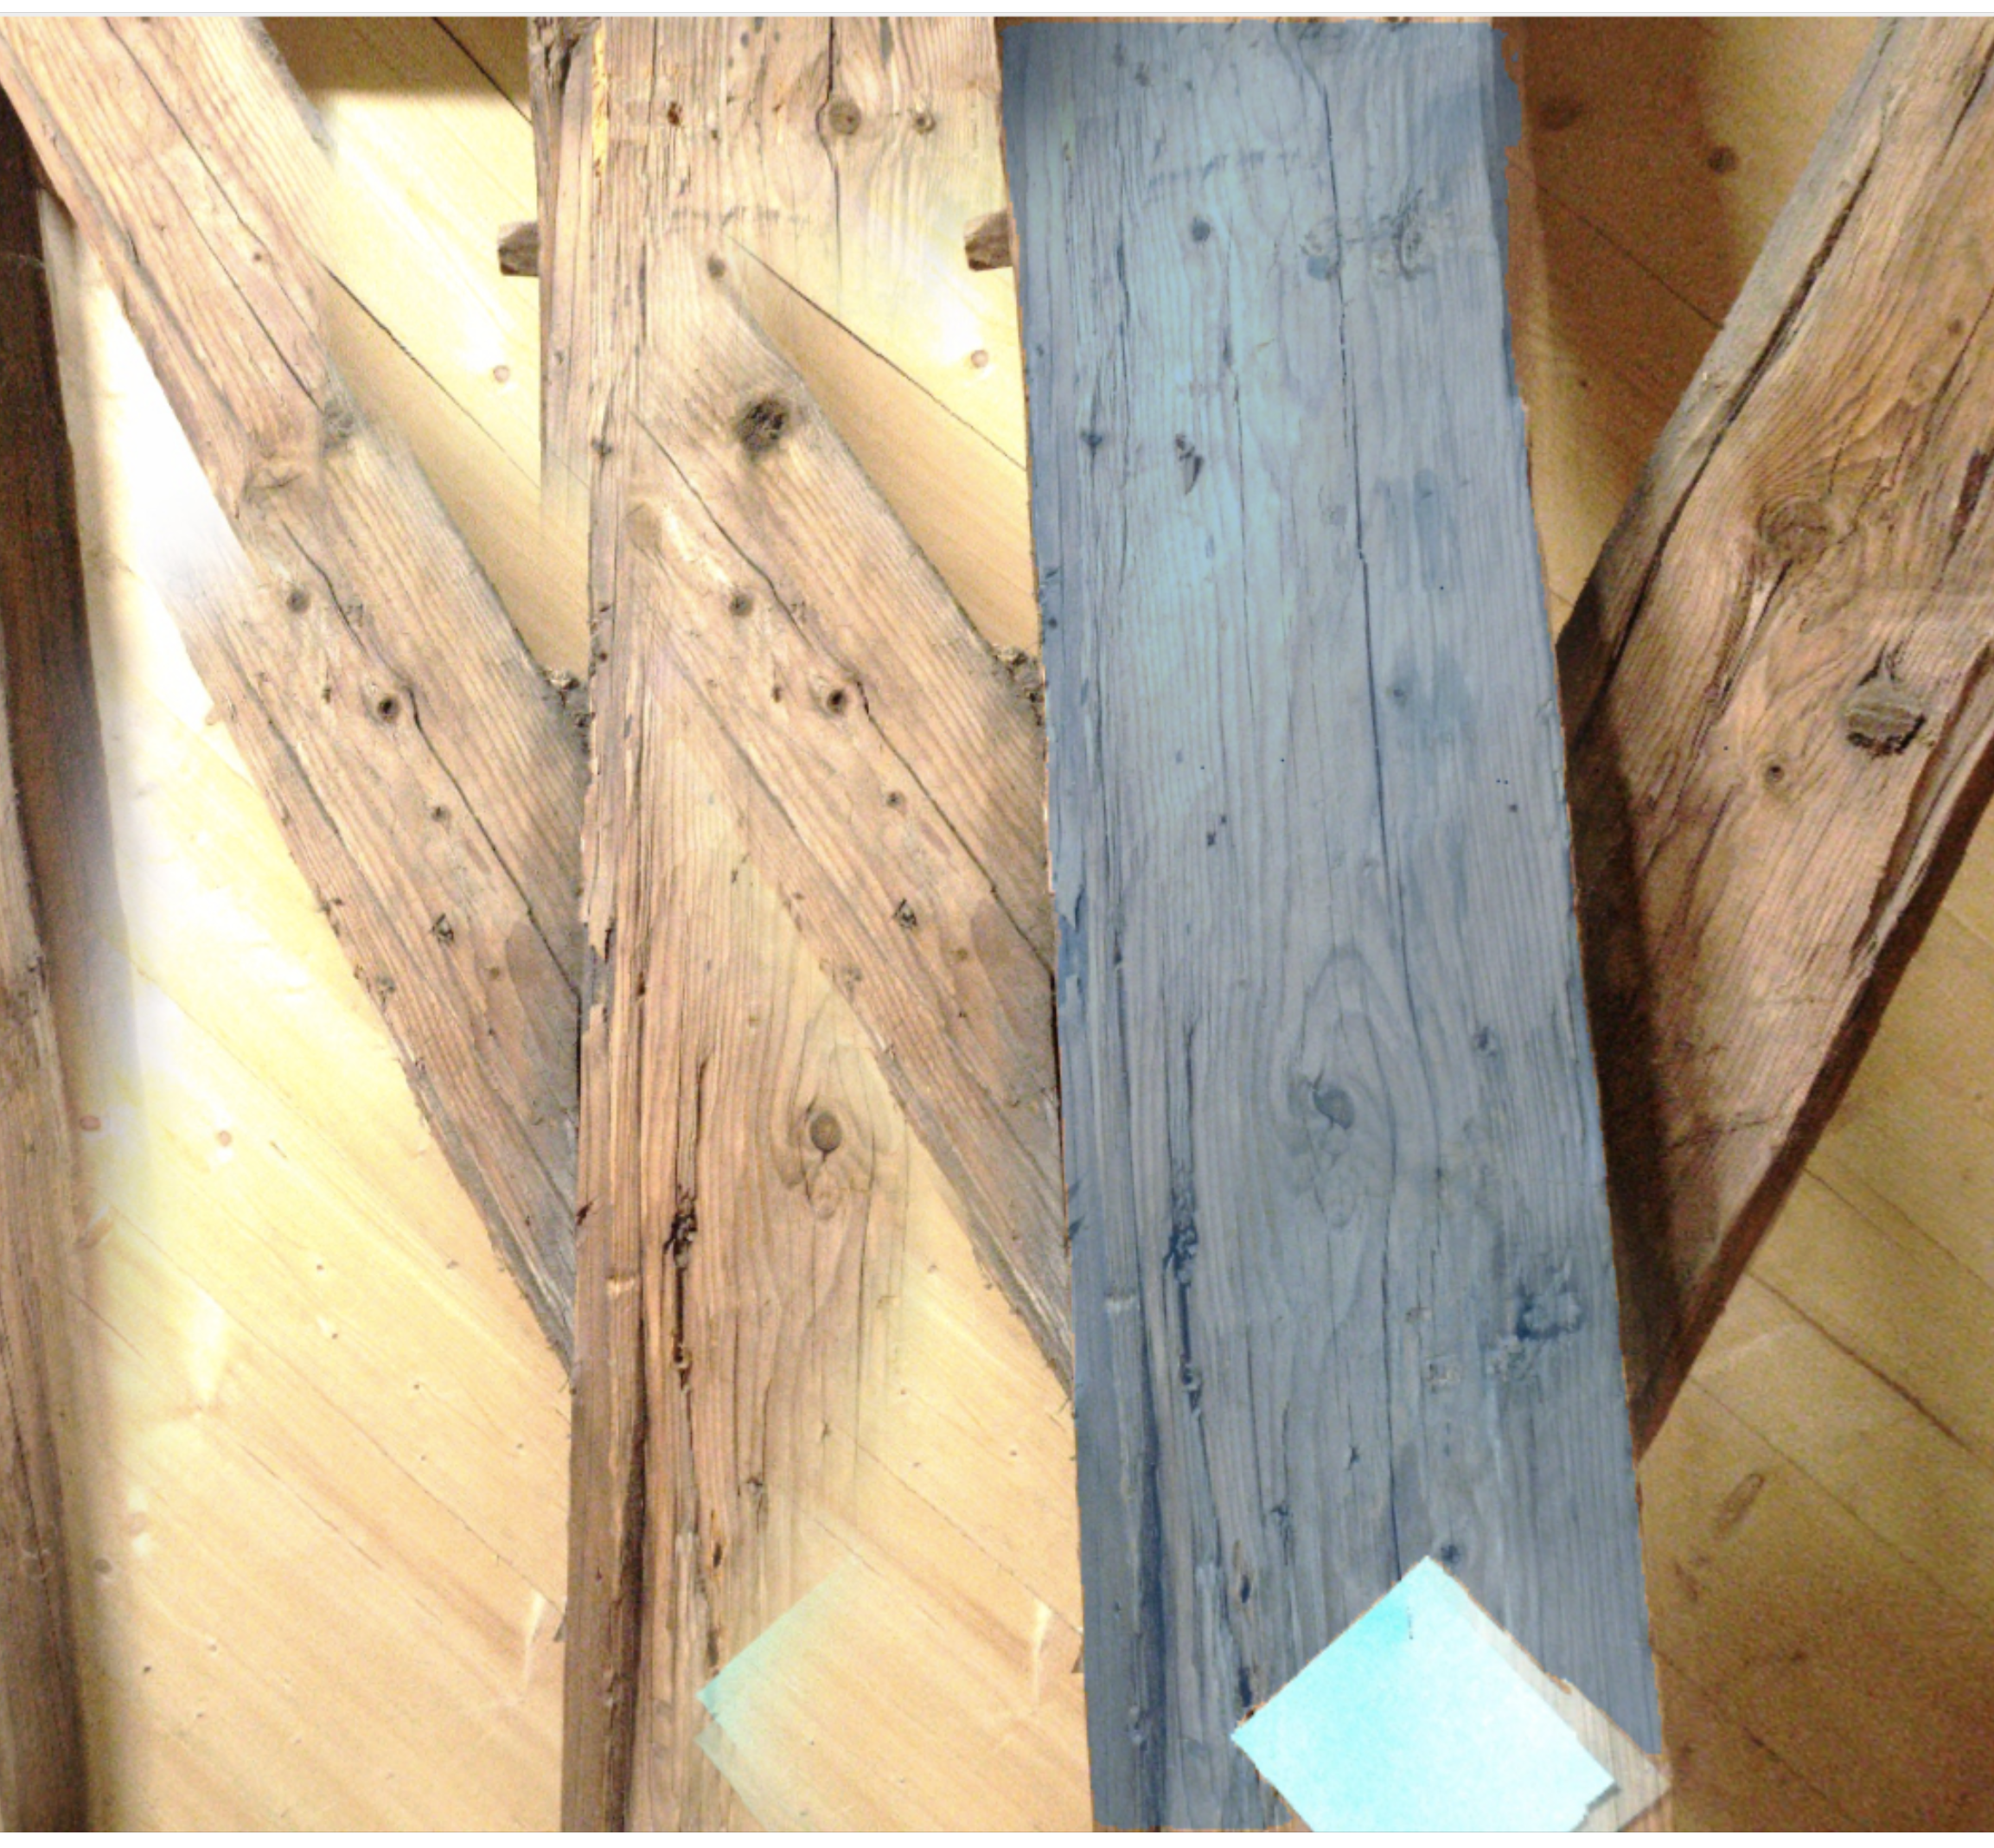
\includegraphics[width=\textwidth,height=4cm,keepaspectratio=false]{Master Thesis/Images/Section_3/SAM/3_sam_test_1.png}
    \end{subfigure}
    \hspace{1cm}
    \begin{subfigure}[b]{0.3\textwidth}
      \centering
        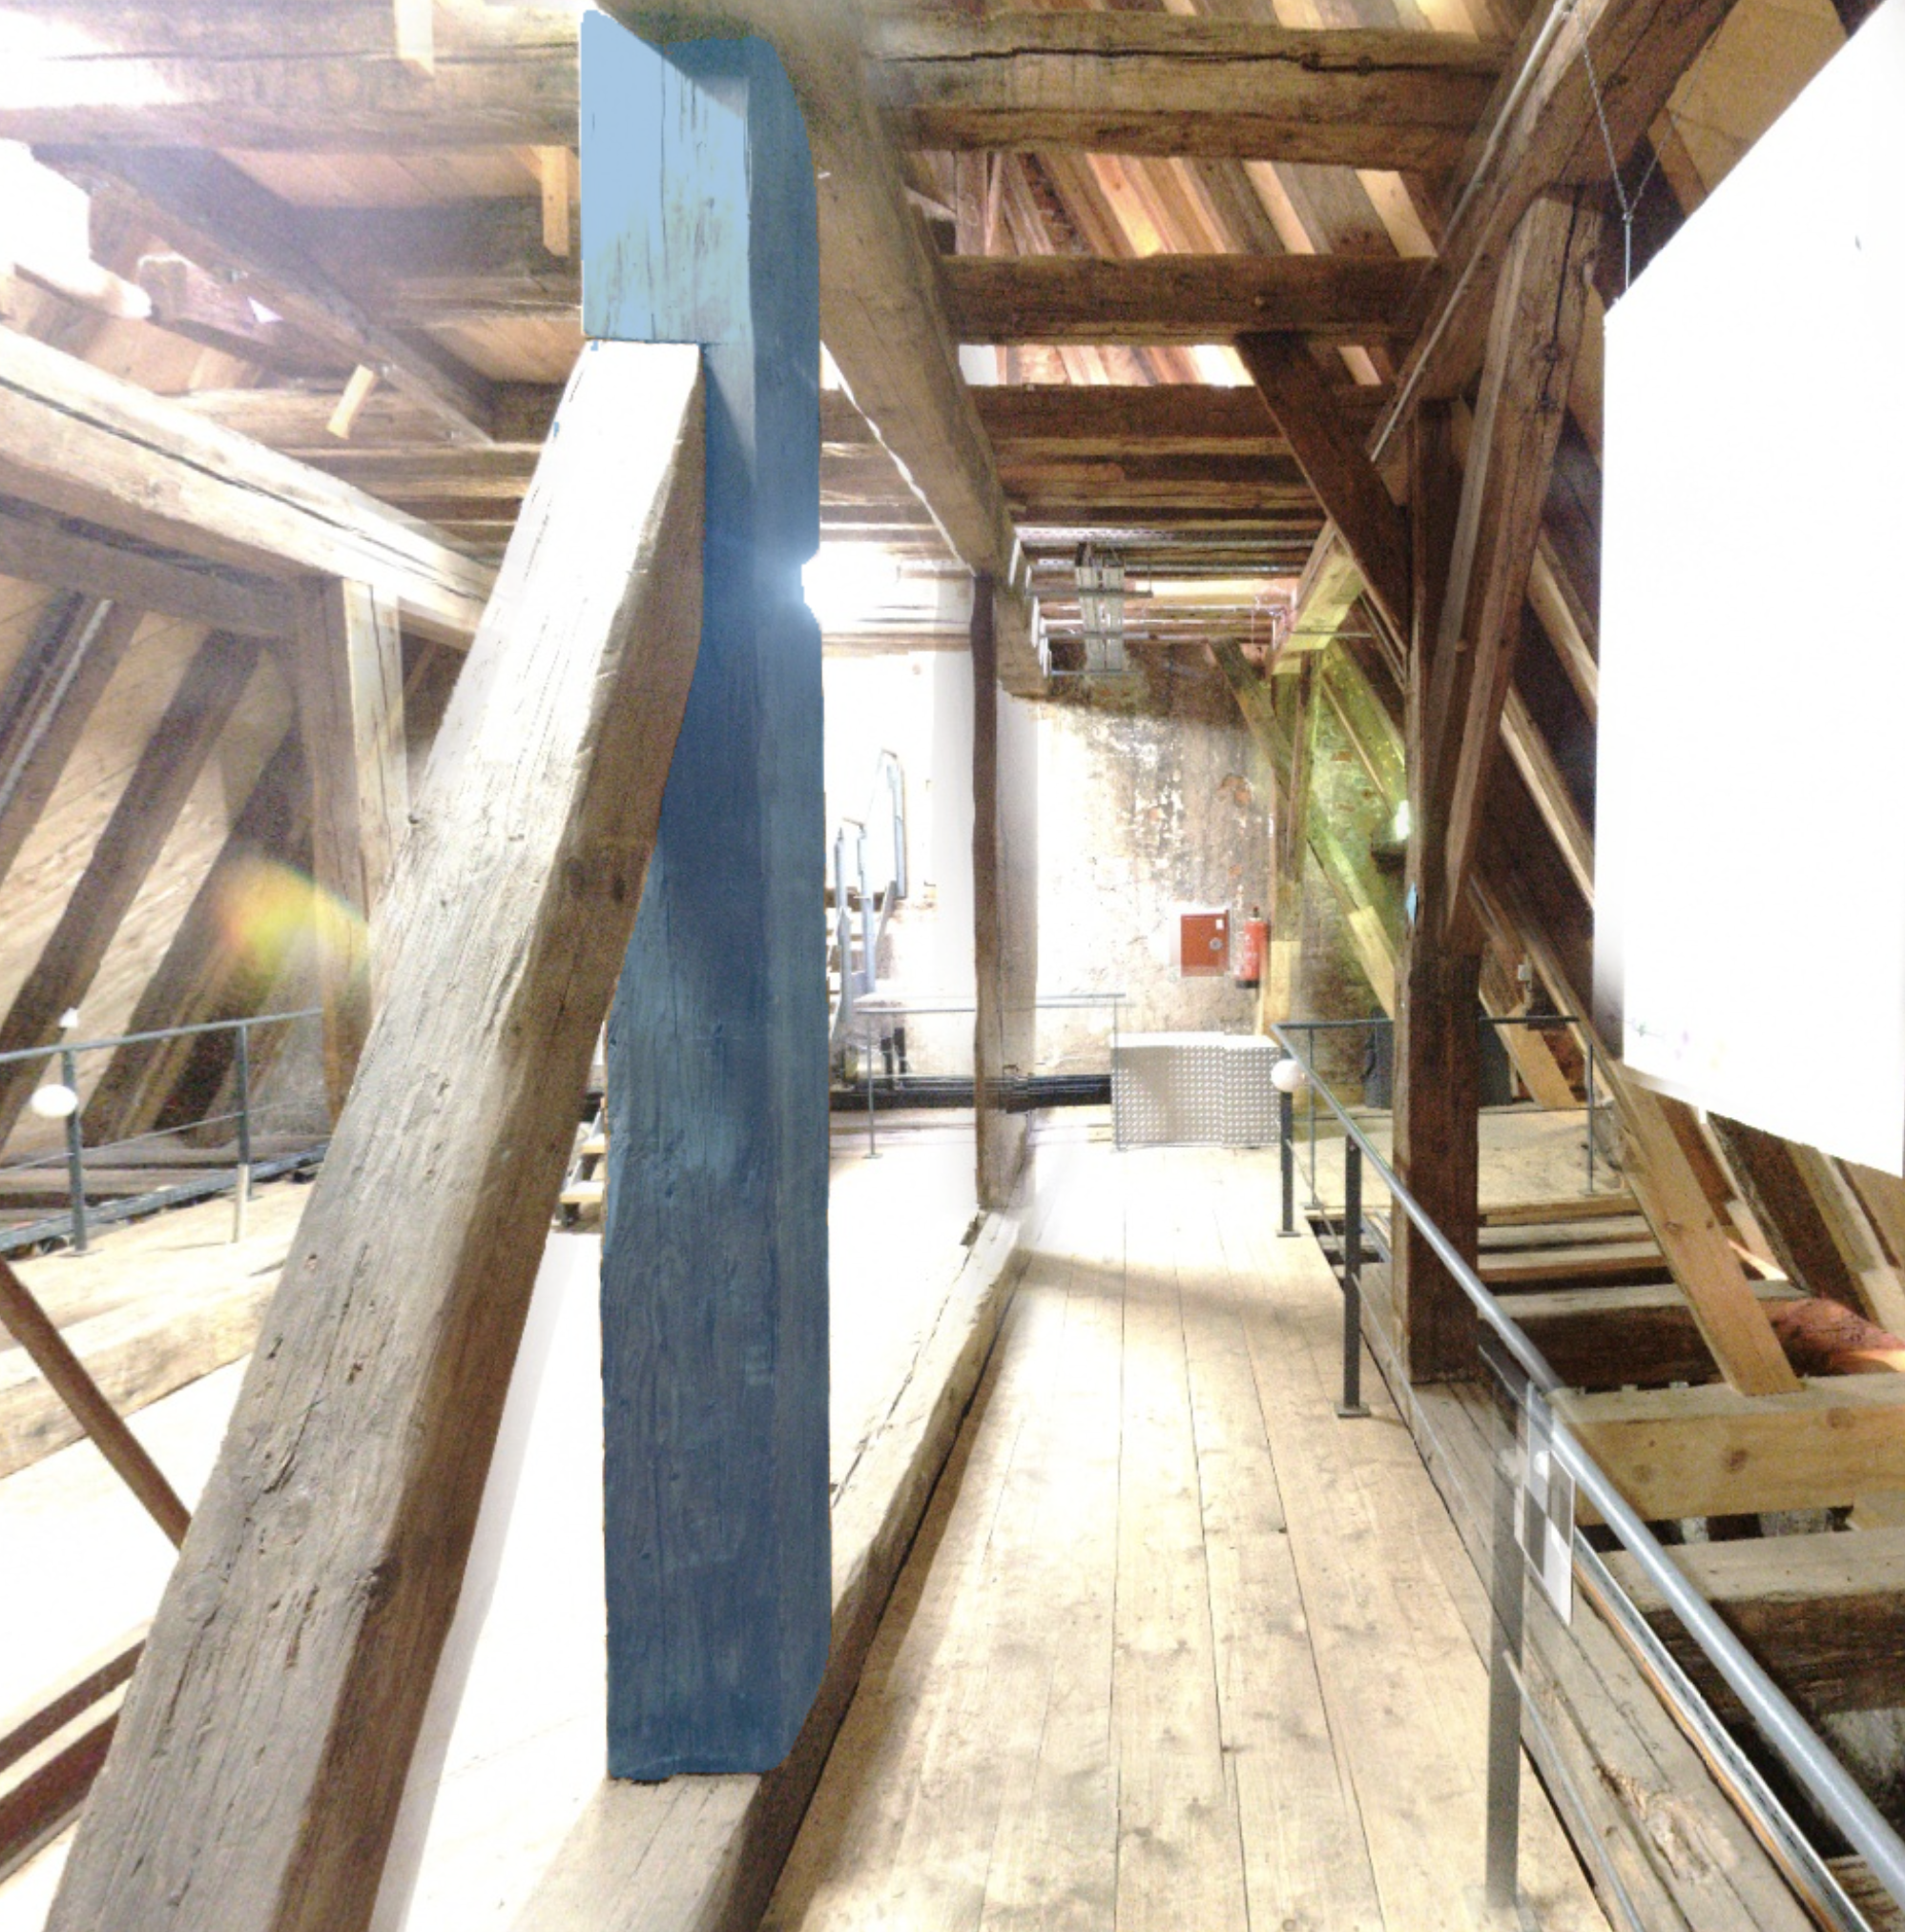
\includegraphics[width=\textwidth,height=4cm,keepaspectratio=false]{Master Thesis/Images/Section_3/SAM/3_sam_test_2.png}
    \end{subfigure}
  \caption{Examples of segmentation on wooden beams using SAM (segment anything)}
\label{fig:sam_test}
\end{figure}

\textbf{Potential methods}:\\
Several models will be considered to achieve a valuable performance for the segmentation. Stat-of-art models like Segment Anything(\cite{kirillov2023segany})(Test in Figure~\ref{fig:sam_test}), Detectron2(\cite{wu2019detectron2}) or Mask R-CNN(\cite{matterport_maskrcnn_2017}) are expected to support this step. However, all models need to be fine-tuned using the mentioned datasets to hopefully segment the main target wooden beams and properly be modified to fit the final workflow.

\hspace*{\fill}

\textbf{Output}:\\
Output will be the segmented single image and position of segmented target area.

\hspace*{\fill}

% \textbf{Potential challenges}:\\
% - \\
% - 313\\
% - qweq\\

\newpage
\subsection{Detection of wood knots}
\label{sec_3:3.2}

\renewcommand\thesection{\arabic{section}}
\renewcommand\thesubsection{\thesection.\arabic{subsection}}



\textbf{Goal}:

This step aims to detect the wood knots on the target surface which will be segmented through the previews process. Ideal output will be shown in Figure~\ref{fig:mock2}.

\hspace*{\fill}

\textbf{Data set}:

An annotated data set of 640 images taken in a wood workshop in Schweinfurt and an unlabelled data set of 296 images from the historic roof construction of the Dominican church in Bamberg are available for the detection of wooden knots. Further datasets based on various historic timber structures are under consideration.

\hspace*{\fill}

\begin{figure}[ht]
  \centering
    \begin{subfigure}[b]{0.4\textwidth}
      \centering
        \includegraphics[width=0.55\textwidth]{Master Thesis/Images/Section_3/Mock/3-Mock2.png}
    \end{subfigure}
    \begin{subfigure}[b]{0.4\textwidth}
      \centering
        \includegraphics[width=0.55\textwidth]{Master Thesis/Images/Section_3/Mock/3-Mock3.png}
    \end{subfigure}
  \caption{Mocked-up output through detection of wooden knots}   
    \label{fig:mock2}
\end{figure}  

\textbf{Potential methods}:

In the earlier experiments, YOLOv8~\citep{yolov8_ultralytics} was used to test the performance of detection on wood knots using the mentioned self-captured dataset (Figure~\ref{fig:yolo_dataset}). The figure~\ref{fig:yolo_results} shows the results within the first experiments, which also show some insufficient bad cases that were wrongly detected. On the other hand, the SSD (single shot multibox detector, \citep{jia2014caffe}) also shows a potentially ideal performance. Both models should be further fine-tuned and optimised. 

\begin{figure}[htbp]
\centering
\begin{minipage}[t]{0.4\linewidth}
\centering
\includegraphics[height=4cm,width=4cm]{Master Thesis/Images/Section_3/Test_YOLO/3-dataset.png}
\caption{\parbox[t]{0.7\textwidth}{Annotated Data set with wood knots in bounding box}}
\label{fig:yolo_dataset}
\end{minipage}%
\hfill
\begin{minipage}[t]{0.6\linewidth}
\centering
\includegraphics[height=4cm,width=4cm]{Master Thesis/Images/Section_3/Test_YOLO/3-007_3679_resize.JPG}
\includegraphics[height=4cm,width=4cm]{Master Thesis/Images/Section_3/Test_YOLO/3-007_3716_resize.JPG}
\caption{\parbox[t]{0.6\textwidth}{Results using YOLOv8m with 100 epochs}}
\label{fig:yolo_results}
\end{minipage}
\end{figure}

\hspace*{\fill}

\textbf{Output}:

The output is an image with the detected knots in bounding box and the position of the bounding box, which should be inside the detected area from previous segmentation process. (Figure~\ref{fig:mock2})




\subsection{Estimation of wood knots}
\label{sec_3:3.3}

\renewcommand\thesection{\arabic{section}}
\renewcommand\thesubsection{\thesection.\arabic{subsection}}


\textbf{Goal}:

Ideally, this step focuses on estimating the dimensions of the wood knots, using the built-in iPhone Measure API and/or a machine learning model to correctly calculate the exact size of the bounding box of the detected wood knots in reality. 


\begin{figure}[ht]
  \centering
   \includegraphics[width=.5\textwidth]{Master Thesis/Images/Section_3/3_iphone_measure.jpg}
  \caption{Mesurement using Measure App in iPhone}   
  \label{fig:iphone_mea}
\end{figure}  

\hspace*{\fill}

\textbf{Dataset}:

The dataset for measurement estimation required a concrete annotation for the pixel-dimensional bounding box in the image and its associated physical dimension. The creation of this specific dataset would only be considered after the insufficient measurement via the iPhone API.

\hspace*{\fill}

\textbf{Potential methods}:

Apple offers various APIs to access data from sensors such as Lidar or Gyroscope. It is also possible to access the measurement API~\footnote{https://developer.apple.com/documentation/foundation/measurement} in the iPhone supported by Apple's ARKit. (Figure~\ref{fig:iphone_mea}) Alternatively, it is also possible to build a machine learning model to estimate the dimension without a sensor. This method would require a large amount of annotated images with the size of the bounding box of wood knots both in pixels and in centimetres, which would be a much more time-consuming task and may also lead to greater bias than using the sensor. 


In conclusion, the first attempt would be to use the API in the iPhone to measure the actual dimension of a standard image and calculate the scale of the conversion from image to actual size. Then it is possible to use the standard image to calibrate the other images that are assumed to have been taken under similar circumstances and calculate the target measurement using the scale.

\hspace*{\fill}

\textbf{Output}:

The output will be one data group for each bounding box, which contains the dimension of the square bounding box and the distance from the border of the bounding box to wooden beam boundary.

\begin{figure}[ht]
    \begin{subfigure}[b]{0.3\textwidth}
        \includegraphics[width=0.7\textwidth]{Master Thesis/Images/Section_3/Mock/3-Mock3.png}
    \end{subfigure}
     \hfill
    \begin{subfigure}[b]{0.3\textwidth}
        \includegraphics[width=0.7\textwidth]{Master Thesis/Images/Section_3/Mock/3-Mock4.png}
    \end{subfigure}
     \hfill
    \begin{subfigure}[b]{0.3\textwidth}
        \includegraphics[width=0.7\textwidth]{Master Thesis/Images/Section_3/Mock/3-Mock5.png}
    \end{subfigure}
  \caption{Mocked-up output after dimension estimation of wood knots and distance to the boundary of wooden beams.}   
    \label{fig:mock3}
\end{figure}  


\newpage

\subsection{Further methods}
\label{sec_3:3.4}

\input{Master Thesis/Parts/3.4_further_methods}

\newpage

\section{Experiments}


\newpage
\section{Analyses}


\newpage
\section{Conclusion}


Some more of your text. For citations, use the command \verb+\citep{lecun2015deep}+ which produces~\citep{lecun2015deep} or \verb+\cite{lecun2015deep}+ which produces~\cite{lecun2015deep}.


Here is a reference to Table~\ref{t1:sample}. Figure~\ref{fig:xai_logo} shows \ldots


\begin{table}[ht]
	\caption{Sample table title}
	\centering
	\begin{tabular}{lll}
		\hline
		Name     & Description     & Size ($\mu$m) \\
		\hline
		Dendrite & Input terminal  & $\sim$100     \\
		Axon     & Output terminal & $\sim$10      \\
		Soma     & Cell body       & up to $10^6$  \\
		\hline
	\end{tabular}
   \label{t1:sample}
\end{table}


\begin{figure}[ht]
  \centering
   \includegraphics[width=.5\textwidth]{xaiLogo.png}
  \caption{Logo of the chair of Explainable Machine Learning}   
  \label{fig:xai_logo}
\end{figure}  

If you want to typeset formulas, there is the inline version $ y = x_1^{0.5} x_2^{0.5}$, centred like this
\[
y = x_1^{0.5} x_2^{0.5}
\]
or numbered:
\begin{equation}\label{eq:prod}
y = x_1^{0.5} x_2^{0.5}	
\end{equation}
so that you can refer to equation~\ref{eq:prod} in the text.


% --------------------------
\clearpage
\begin{appendix}
	\section{Appendix}
	If needed for supplementary material, such as detailed description of data collection, tables, or figures.
	
\end{appendix}

% ----------------------------------------------------------------------------
% Bibliography
% ----------------------------------------------------------------------------
\clearpage
\renewcommand\refname{Bibliography}
\addcontentsline{toc}{section}{Bibliography}
\bibliography{bibliography}
\bibliographystyle{plainnat}

% ----------------------------------------------------------------------------
% Statutory declaration
% ----------------------------------------------------------------------------
\clearpage
\makeThesisDeclaration

\end{document}

